%% Classe du document
\documentclass[a4paper,10pt]{article}

%% Francisation
\usepackage[francais]{babel} % Indique que l'on utilise le francais
\usepackage[T1]{fontenc}
\usepackage[utf8]{inputenc} % Indique que l'on utilise tout le clavier
%\usepackage[latin1]{inputenc}

%% Réglages généraux
\usepackage[top=3cm, bottom=3cm, left=3cm, right=3cm]{geometry} % Taille de la feuille
\usepackage{lastpage}

%% Package pour le texte
\usepackage{soul} % Souligner
\usepackage{color} % Utilisation de couleurs
\usepackage{hyperref} % Créer des liens et des signets
\usepackage{eurosym}% Pour le symbole euro
\usepackage{fancyhdr}% Entête et pied de page

%% Package pour les tableaux
\usepackage{multirow} % Colonnes multiples
\usepackage{cellspace}
\usepackage{array}

%% Package pour les dessins
\usepackage{pstricks}
\usepackage{graphicx} % Importer des images
\usepackage{pdftricks} % Pour utiliser avec pdfTex
\usepackage{pst-pdf} % Pour utiliser avec pdfTex
\usepackage{pst-node} % Pose de noeuds
\usepackage{subfig}
\usepackage{float}

%% Package pour les maths
\usepackage{amsmath} % Commandes essentielles
\usepackage{amssymb} % Principaux symboles

%% Package pour le code
\usepackage{listings} % Utilisation de la couleur syntaxique des langages
\usepackage{url}


\usepackage[babel=true]{csquotes} % Permet les quotations (guillemets)
\usepackage{tocvsec2}
\usepackage{amsthm}
\usepackage{amsfonts}

\usepackage{tikz}
\usepackage{pdfpages}

\usetikzlibrary{shapes} % A revoir

%--------------------- Autres définitions ---------------------%

% Propriété des liens
\hypersetup{
colorlinks = true, % Colorise les liens
urlcolor = blue, % Couleur des hyperliens
linkcolor = black, % Couleur des liens internes
}

\definecolor{grey}{rgb}{0.95,0.95,0.95}

% Language Definitions for Turtle
%TODO: a revoir avec les couleur de gedit
\definecolor{olivegreen}{rgb}{0.2,0.8,0.5}
\definecolor{grey2}{rgb}{0.5,0.5,0.5}
\lstdefinelanguage{ttl}{
sensitive=true,
morecomment=[s][\color{grey2}]{@}{:},
morecomment=[l][\color{olivegreen}]{\#},
morecomment=[s][\color{red}]{<}{/>},
morestring=[s][\color{olivegreen}]{<http://w}{\#>},
morestring=[b][\color{blue}]{\"},
}

\lstset{
frame=single,
breaklines=true,
basicstyle=\ttfamily,
backgroundcolor=\color{grey},
basicstyle=\scriptsize,
keywordstyle=\color{blue},
commentstyle=\color{green},
stringstyle=\color{red},
identifierstyle=\color{blue}
}

%Definition de la commande pour retirer l'espace devant les ':'
\makeatletter
\@ifpackageloaded{babel}%
        {\newcommand{\nospace}[1]{{\NoAutoSpaceBeforeFDP{}#1}}}%  % !! double {{}} pour cantonner l'effet à l'argument #1 !!
        {\newcommand{\nospace}[1]{#1}}
\makeatother

\setcounter{tocdepth}{3}
%\maxsecnumdepth{subsubsection} % Dernière section numérotée

\newcommand{\paperPrototyping}{\emph{paper prototyping}}

% Corps du document :
\begin{document}

% Définition des entêtes et pieds de page
\fancyhead[LE,CE,RE,LO,CO,RO]{}
\fancyfoot[LE,CE,RE,LO,CO,RO]{}
\fancyhead[LO, LE]{Interface Homme-Machine 2}
\fancyhead[RO,RE]{2012/2013}
\fancyfoot[LO,LE]{Université de \scshape{Nantes}}
\fancyfoot[RO,RE]{Page \thepage \ sur \pageref{LastPage}}
\renewcommand{\headrulewidth}{0.4pt}
\renewcommand{\footrulewidth}{0.4pt}

%\maketitle
\begin{titlepage}

\vspace*{\fill}~
\begin{center}
{\large \textsc{Rapport de Projet}} \\
\vspace{1cm}
{\LARGE Projet : Gestionnaire simple de tâches} \\
\vspace{1cm}
\textbf{Taskinator Android} \\
\vspace{0.3cm}

\includegraphics[height=1cm]{Images/Taskinator.png} 
\includegraphics[height=1cm]{Images/android.png} \\
\vspace{1cm}
COUTABLE Guillaume, RULLIER Noémie \\
\today
\end{center}
\vspace*{\fill}

\vspace{\stretch{1}}
\begin{center}
\noindent 

\includegraphics[height=2.5cm]{Images/universite.png}
\end{center}
\pagebreak
\end{titlepage}

\newpage
\tableofcontents  

% Introduction
\newpage
\pagestyle{fancy}

%%%%%%%%%%%%%%%%%%%%%%%%%%%%%%%%%%%%%%%%%%%%%%%%%%%%%%%%%%%%%%%%%%%%%%%%%%%%%
%%%%%%%%%%  Introduction générale
%%%%%%%%%%%%%%%%%%%%%%%%%%%%%%%%%%%%%%%%%%%%%%%%%%%%%%%%%%%%%%%%%%%%%%%%%%%%%
\section{Introduction}
L'objectif de ce projet fut de développer un gestionnaire simple de tâches. Celui-ci devait permettre de créer des listes de tâches et de suivre l'avancement de celles-ci.

Afin de créer cette application que nous avons appelé \textit{Taskinator}, nous avons établit plusieurs étapes dans l'avancement du projet. Ce rapport présentera ces étapes les unes après les autres.

%%%%%%%%%%%%%%%%%%%%%%%%%%%%%%%%%%%%%%%%%%%%%%%%%%%%%%%%%%%%%%%%%%%%%%%%%%%%%
%%%%%%%%%%  Etape 1
%%%%%%%%%%%%%%%%%%%%%%%%%%%%%%%%%%%%%%%%%%%%%%%%%%%%%%%%%%%%%%%%%%%%%%%%%%%%%
\newpage
\section{Les fonctionnalités}
La première étape fut d'analyser l'ensemble des fonctionnalités que notre application devait proposer. 

\subsection{Fonctionnalités principales}
Voici dans un premier temps les fonctionnalités principales:
\paragraph{Créer une liste:} cette fonctionnalité permet à l'utilisateur de créer une liste vide.
\paragraph{Créer une tâche:} cette fonctionnalité permet à l'utilisateur de créer une tâche.
\paragraph{Supprimer un élément:} cette fonctionnalité permet de supprimer une tâche ou une liste. Cette fonctionnalité est à manipuler avec précaution, en effet dans le cas d'une liste, la suppression de celle-ci implique aussi la suppression de toutes ses tâches.

\subsection{Fonctionnalités secondaires}
Voici les fonctionnalités secondaires:
\paragraph{Monter / Descendre:} cette fonctionnalité permet de monter ou descendre une liste ou une tâche. Dans le cas d'une liste, toutes ces tâches sont aussi montées/descendues d'un rang. Dans le cas d'une tâche, on autorise un déplacement dans une autre liste. (Cette fonctionalité n'a pas été implémentée)

%%%%%%%%%%%%%%%%%%%%%%%%%%%%%%%%%%%%%%%%%%%%%%%%%%%%%%%%%%%%%%%%%%%%%%%%%%%%%
%%%%%%%%%%  Etape 2
%%%%%%%%%%%%%%%%%%%%%%%%%%%%%%%%%%%%%%%%%%%%%%%%%%%%%%%%%%%%%%%%%%%%%%%%%%%%%
\newpage
\section{Scénarios}
Nous avons imaginé différents scénarios d'utilisation de notre application.

\subsection{Scénario 1 - Création/Utilisation/Suppression d'une liste}
Ce premier scénario permet de créer une liste et d'y ajouté des tâches.
\begin{enumerate}
\item{L'utilisateur crée une liste et lui donne un nom \textit{Ski}.}
\item{Il crée ensuite une tâche dans cette liste et lui donne un nom \textit{Bonnet}.}
\item{Il crée ensuite une autre tâche dans cette liste et lui donne un nom \textit{Echarpe}.}
\item{L'utilisateur supprime la tâche \textit{Bonnet}.}
\item{L'utilisateur supprime la liste \textit{Ski}. Une popup apparaît pour l'avertir que cette suppression supprimera aussi toutes les tâche de la liste.}
\end{enumerate}

\subsection{Scénario 2 - Gestion des listes et sauvegarde}
Ce scénario permet de créer des listes et de les modifiers. Il permet aussi de constater que l'état de l'application est sauvegardé.
\begin{enumerate}
\item{L'utilisateur choisit de créer une liste et lui donne un nom \textit{Course}.}
\item{Il décide ensuite de créer une nouvelle liste et lui donne un nom \textit{Sac de voyage}.}
\item{Il décide ensuite d'inverser ces deux listes, pour cela il reste longtemps appuyé sur la liste \textit{Sac de voyage} et la glisse un rang plus haut.}
\item{L'utilisateur va ensuite supprimer la liste \textit{Course}.}
\item{L'utilisateur va ensuite ouvrir une autre application et revenir sur \textit{Taskinator}. Il peut constater que l'application est ouverte avec l'état dans lequel on l'a quittée. C'est à dire que si une liste était ouverte ou fermée quand on a quitté l'application, celle-ci sera dans le même état quand on y reviendra.}
\item{L'utilisateur décide de créer une nouvelle tâche dans \textit{Sac de voyage}. Pendant qu'il entre le nouveau nom de cette tâche, il va recevoir un appel. Lorsque l'appel est terminé, il sera automatiquement redirigé vers Taskinator exactement dans le même état qu'avant l'appel. S'il avait commencé à taper \textit{Chauss}, il retrouvera le même début de mot.}
\item{L'utilisateur va recevoir un appel pendant qu'il est en train de rentrer un nom pour sa liste}
\item{Cette fois-ci, l'utilisateur quitte l'application. De même s'il l'a lance à nouveau, celle-ci est ouverte avec le dernier état dans lequel on l'a quittée.}
\end{enumerate}


%%%%%%%%%%%%%%%%%%%%%%%%%%%%%%%%%%%%%%%%%%%%%%%%%%%%%%%%%%%%%%%%%%%%%%%%%%%%%
%%%%%%%%%%  Etape 3
%%%%%%%%%%%%%%%%%%%%%%%%%%%%%%%%%%%%%%%%%%%%%%%%%%%%%%%%%%%%%%%%%%%%%%%%%%%%%
\newpage
\section{L'IHM}

\subsection{L'activité principale}
L'application est tout simplement composée d'une zone réservée à l'affichage de la liste en cours de création et d'une barre d'action.
\begin{figure}[H]
    \center
    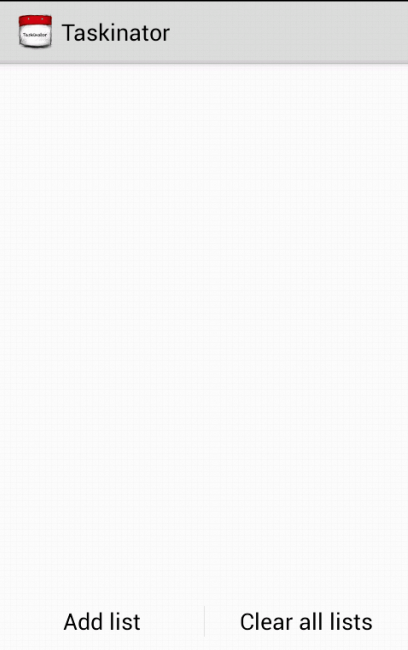
\includegraphics[width=3.7cm]{Images/mainActivity.png}\quad
    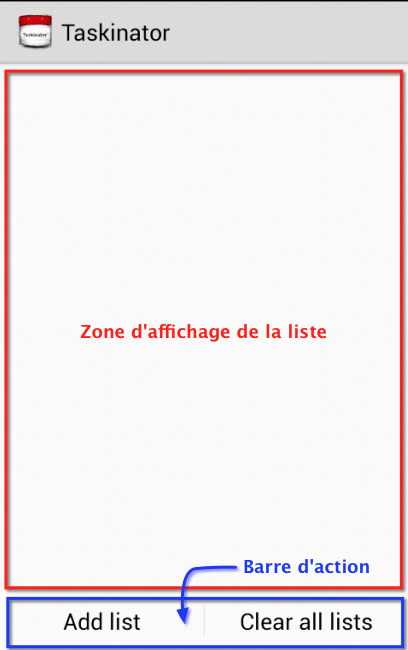
\includegraphics[width=3.7cm]{Images/mainActivityPart.png}
    \caption{L'application}
\end{figure}

\subsubsection{Choix réalisés (Position des boutons, Gestures, ...)}
Dans cette section, nous expliquons les choix effectués et pourquoi nous avons choisi de mettre en place ces solutions:

\begin{itemize}
\item \textbf{Fonctionnalité de création de liste:} nous avons choisi de créer de nouvelles listes en cliquant sur le bouton "Add list" en bas de l'écran.
\begin{figure}[H]
    \center
    \subfloat[Boîte de dialogue pour le nom de la liste]{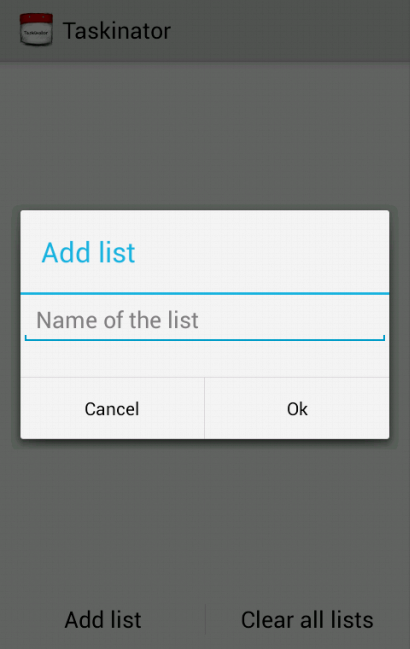
\includegraphics[width=3.7cm]{Images/addList.png}}\quad
    \subfloat[Liste vide fermée]{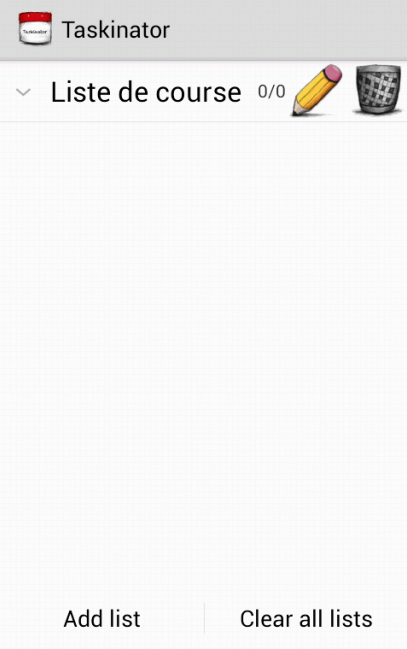
\includegraphics[width=3.7cm]{Images/enteteList.png}}\quad
    \subfloat[Liste vide ouverte]{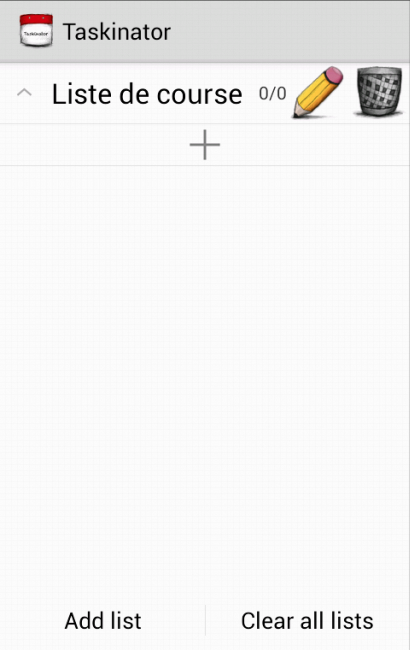
\includegraphics[width=3.7cm]{Images/listVide.png}}
    \caption{Ajout d'une liste}
\end{figure}
Une boite de dialogue apparaît et permet de rentrer le nom de cette nouvelle liste. L'utilisateur doit ensuite valider en cliquant sur "OK", s'il appui sur "Cancel", la nouvelle liste ne sera pas créée. Si l'utilisateur déroule sa liste, un nouvel item apparaît sur la page muni d'un bouton "+". Celui-ci permettra de créer de nouvelles tâches pour la liste.
\item \textbf{Fonctionnalité de création de tâche:} nous avons choisi de créer de nouvelles tâches en cliquant sur le bouton "+" présent sous chaque liste pour ajouter une tâche à la liste correspondante. Lorsque l'utilisateur clique sur ce bouton, une nouvelle boite de dialogue apparaît et permet de rentrer le nouveau nom de la tâche.
\begin{figure}[H]
    \center
    \subfloat[Boîte de dialogue pour le nom de la tâche]{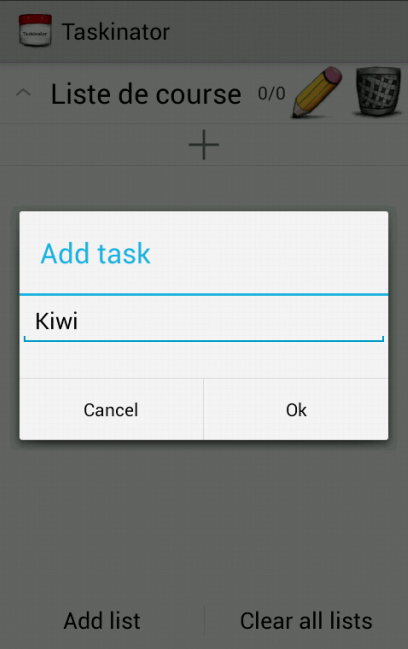
\includegraphics[width=3.7cm]{Images/addTask.png}}\quad
    \subfloat[Tâche]{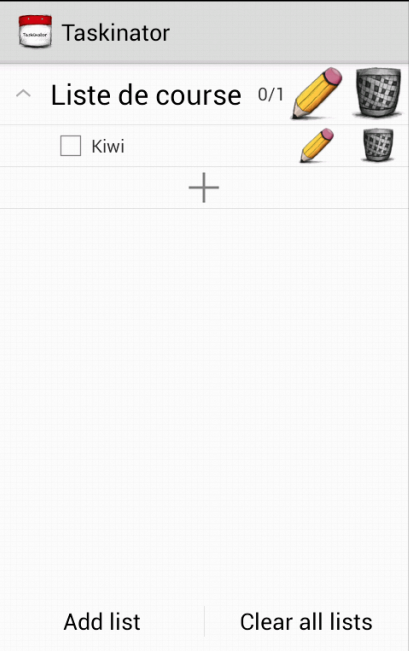
\includegraphics[width=3.7cm]{Images/listTask.png}}
    \caption{Ajout d'une tâche}
\end{figure}
L'utilisateur doit valider l'ajout en cliquant sur "OK". Un nouvel item de tâche apparaît dans la liste (au-dessus du bouton "+"). Nous avons choisi de procéder ainsi plutôt que de mettre un bouton de création dans l'entête de la liste, pour éviter à l'utilisateur de remonter en haut de la liste à chaque fois qu'il souhaite ajouter une tâche (cela peut vite devenir contraignant).
\item \textbf{Fonctionnalité \textit{Monter} et \textit{Descendre}:} nous avons décidé d'accéder à cette fonctionnalité seulement grâce aux gestures. En effet, il suffit à l'utilisateur de rester longtemps appuyer sur une liste ou tâche et de la glisser à l'endroit voulu. (Fonctionnalitée non implémentée mais expérimentée voir \ref{experimentation}).
\item \textbf{Fonctionnalité \textit{Modifier}:} nous avons choisi d'ajouter cette possibilité de modification du nom sur chaque élément par la présence du bouton 
\includegraphics[width=0.5cm]{Images/modify.png}.
\item \textbf{Fonctionnalité \textit{Supprimer}:} nous avons choisi d'ajouter cette possibilité de suppression sur chaque élément (liste ou tâche) pour que l'utilisateur puisse supprimer plus rapidement. De  plus nous avons décidé de faire apparaître une fenêtre d'avertissement car la suppression d'une liste entraîne la suppression de toutes ses tâches. Le bouton représentant cette fonctionnalité est le suivant 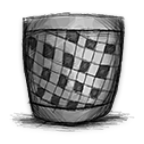
\includegraphics[width=0.5cm]{Images/trash_empty.png}
\item \textbf{Fonctionnalité \textit{Supprimer tout}:} nous avons choisi d'ajouter cette possibilité de supprimer l'ensemble des listes crées par l'utilisateur afin que celui-ci n'est pas à supprimer toutes les tâches une par une s'il souhaite vraiment tout supprimer. De  plus nous avons décidé de faire apparaître une fenêtre d'avertissement car la suppression de l'ensemble des listes est une opération importante.
\item \textbf{Indicateur:} nous avons choisi d'ajouter sur la liste un indicateur permettant de connaître le nombre de tâches validées sur le nombre de tâche de la liste, afin que l'utilisateur puisse voir l'état de sa liste plus rapidement.
\begin{figure}[H]
    \center
    \subfloat[Tâche validée]{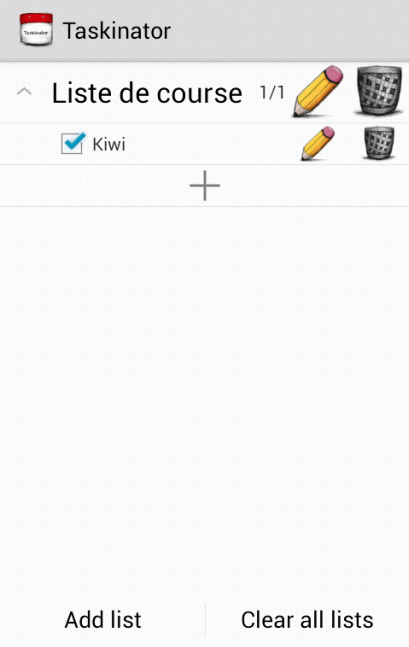
\includegraphics[width=3.7cm]{Images/listTaskChecked.png}} \quad
    \subfloat[Une tâche validée sur deux]{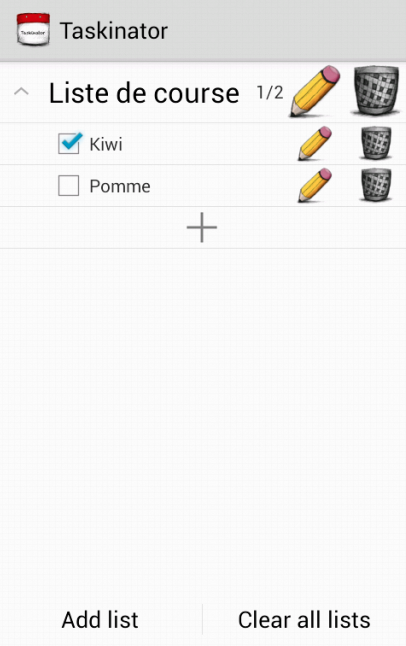
\includegraphics[width=3.7cm]{Images/listTwoTask.png}}
    \caption{Validation de tâche et indicateur}
\end{figure}
\end{itemize}

\subsection{Affichage des listes et tâches}
Afin d'afficher l'ensemble des listes créées et de leur(s) tâche(s), on a décider d'utiliser ExpandableListView, permettant d'afficher l'ensemble des listes et pour chacune d'entre elle sa ou ses tâche(s).

La liste est décrite à l'aide du xml list.xml et est représentée par un TextView permettant d'afficher le nom de celle-ci, d'un autre TextView permettant d'afficher le nombre de tâches validées sur le nombre de tâche de la liste, d'un ImageButton permettant d'ajouter la fonctionnalité de modification du nom de la liste et d'un ImageButton permettant d'ajouter la fonctionnalité de suppression de liste.

La tâche est décrite par le fichier task.xml et est représentée par une checkbox, un TextView permettant de taper d'afficher le nom de la tâche, d'un ImageButton permettant d'ajouter la fonctionnalité de modification du nom sur la tâche et d'un ImageButton permettant d'ajouter la fonctionnalité de suppression sur la tâche.

%%%%%%%%%%%%%%%%%%%%%%%%%%%%%%%%%%%%%%%%%%%%%%%%%%%%%%%%%%%%%%%%%%%%%%%%%%%%%
%%%%%%%%%%  Etape 4
%%%%%%%%%%%%%%%%%%%%%%%%%%%%%%%%%%%%%%%%%%%%%%%%%%%%%%%%%%%%%%%%%%%%%%%%%%%%%
\newpage
\section{Le modèle}
Afin de réaliser cette application nous nous sommes basés sur le modèle suivant dont voici le diagramme de classes:
\begin{figure}[htpb]
	\center
	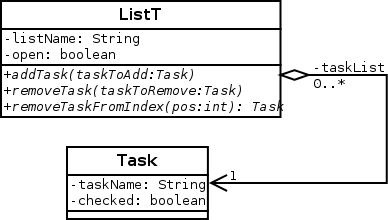
\includegraphics[scale=0.5]{Images/dia_classe.png}
	\caption{Diagramme de classe du modèle}
\end{figure}

Le modèle de cette application est très simple. Il est composé de deux classes, \textit{ListT} et \textit{Task}.
Nous avons donc ici une \textit{ListT} qui va pouvoir contenir un ensemble de tâches et d'autres propriétés comme le nom et si elle est ouverte ou non. Nous avons de plus une \textit{Task} qui va elle représenter une tâche et contenir certaines informations comme son nom et si elle est cochée ou non.
Nous pouvons donc gérer tous ces listes au sein de ce modèle et ainsi, ajouter une tâche dans celle-ci. On peut pour les listes comme les tâches les supprimer, les déplacer d'un rang (dans les deux sens).

%%%%%%%%%%%%%%%%%%%%%%%%%%%%%%%%%%%%%%%%%%%%%%%%%%%%%%%%%%%%%%%%%%%%%%%%%%%%%
%%%%%%%%%%  Etape 5
%%%%%%%%%%%%%%%%%%%%%%%%%%%%%%%%%%%%%%%%%%%%%%%%%%%%%%%%%%%%%%%%%%%%%%%%%%%%%
\newpage
\section{Sauvegarde des données}
Afin que l'utilisateur retrouve l'ensemble de ses données quand il quitte l'application, ou qu'il tourne son téléphone et que l'orientation change, ou qu'il reçoive un appel pendant qu'il utilise l'application; il a été nécessaire de sauvegarder ses données. Pour cela, nous avons décider d'utiliser l'Internal Storage. Celui-ci permet de stocker en interne des fichiers sur l'appareil et que ces fichiers soit privés pour notre application. Ces fichiers seront supprimés lors de la désinstallation de l'application par l'utilisateur.

Nous avons donc décidé de sauvegarder notre liste dans un fichier \emph{xml} et de la restaurer via ce ficher. Cette sauvegarde s'effectue dans la fonction \emph{onPause()}. Comme on peut le voir sur le schéma ci-dessous, dès que l'activité n'est plus au premier plan, elle passe par la fonction \emph{onPause()}. On est donc sûr d'avoir la dernière version de la liste enregistrée.
Nous devons donc maintenant restaurer cette liste à partir du fichier (que nous avons décidé d'appeler \textit{save.xml}). Nous avons décidé d'effectuer cette restauration dans la fonction \emph{onCreate()}. En effet à chaque nouveau lancement de l'application, on recharge la liste à partir du fichier \textit{save.xml}.
\begin{figure}[htpb]
	\center
	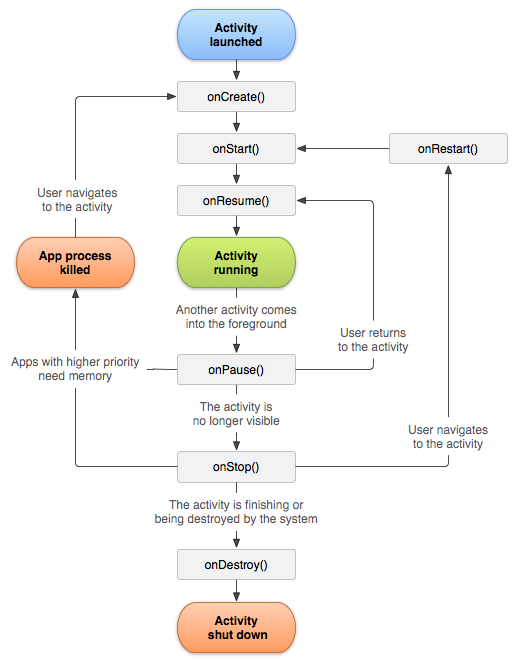
\includegraphics[scale=0.5]{Images/activity_lifecycle.png}
	\caption{Le cycle de vie d'une activité}
\end{figure}

Afin d'enregistrer cette liste dans le fichier \emph{xml}, nous avons créer notre propre parseur.
%TODO Guillaume explication sauvegarde grâce au parseur

%%%%%%%%%%%%%%%%%%%%%%%%%%%%%%%%%%%%%%%%%%%%%%%%%%%%%%%%%%%%%%%%%%%%%%%%%%%%%
%%%%%%%%%%  Etape 6
%%%%%%%%%%%%%%%%%%%%%%%%%%%%%%%%%%%%%%%%%%%%%%%%%%%%%%%%%%%%%%%%%%%%%%%%%%%%%
\newpage
\section{Expérimentation}
\label{experimentation}
%TODO Guillaume

\subsection{Suppression par Swipe}

\subsection{Déplacement de listes/tâches par Drag and Drop}


%%%%%%%%%%%%%%%%%%%%%%%%%%%%%%%%%%%%%%%%%%%%%%%%%%%%%%%%%%%%%%%%%%%%%%%%%%%%%
%%%%%%%%%%  Etape 7
%%%%%%%%%%%%%%%%%%%%%%%%%%%%%%%%%%%%%%%%%%%%%%%%%%%%%%%%%%%%%%%%%%%%%%%%%%%%%
\newpage
\section{Limite de l'application}
Notre application à ses propres limites.
On pourrait imaginer d'ajouter certaines fonctionnalitées comme par exemple:
\begin{itemize}
\item Recherche (
\includegraphics[scale=0.2]{Images/search.png}): qui permetterai à l'utilisateur d'afficher seulement les listes qui ont un nom ou qui ont des tâches dont le nom contient la chaîne du filtre.
\item Partage (
\includegraphics[scale=0.2]{Images/share.png}): qui permettrai à l'utilisateur de partager sa ou ses listes sur des réseaux sociaux ou par mail.
\item Favoris (
\includegraphics[scale=0.2]{Images/favorite.png}): qui permetterai à l'utilisateur de mettre certaines listes ou tâches en favoris et d'y avoir accès via un onglet favoris. Cela permetterai d'avoir un accès plus rapide.
\item Rappel (
\includegraphics[scale=0.2]{Images/event.png}): qui permetterai à l'utilisateur de définir un rappel sur une tâche afin que celle-ci soit exécutée dans les temps.
\end{itemize}
%TODO A compléter si des idées

%%%%%%%%%%%%%%%%%%%%%%%%%%%%%%%%%%%%%%%%%%%%%%%%%%%%%%%%%%%%%%%%%%%%%%%%%%%%%
%%%%%%%%%%  CONCLUSION GENERALE
%%%%%%%%%%%%%%%%%%%%%%%%%%%%%%%%%%%%%%%%%%%%%%%%%%%%%%%%%%%%%%%%%%%%%%%%%%%%%
\newpage
\section{Conclusion générale}
Ce projet nous a permis de réfléchir à la structure de l'IHM afin que celle-ci soit la plus intuitive possible pour l'utilisateur. Réfléchir à la position des
boutons, le nom ou l'icône les représentant, comment l'ajout des composants se fera au sein de la liste, la gesture à utiliser, l'utilisation d'un menu \ldots{}
Et donc, d'orienter notre conception sur l'IHM, plus que sur le modèle, et ainsi expérimenter une autre approche de conception.

\end{document}